\section{Konzeption und Umsetzung des Assistenzsystems}

\subsection{Funktionsumfang und Architektur}
Im Rahmen dieser Projektarbeit wurde ein webbasiertes Assistenzsystem zur
\ac{KI}-gestützten Generierung von Black-Box-Testfällen entwickelt.
Das Ziel des Assistenzsystems ist es, aus der Beschreibung einer
Programmieraufgabe automatisiert Black-Box-Testfälle abzuleiten. Als
Informationsgrundlage dient die Aufgabenbeschreibung oder die Spezifikation eines Programms
und die Eingabebeschränkungen, die definieren, welche Parameter als Input für das Programm erlaubt sind.
Abbildung~\ref{fig:systemablauf} verdeutlicht den Ablauf der Anwendung.

\begin{figure}[h]
    \centering
    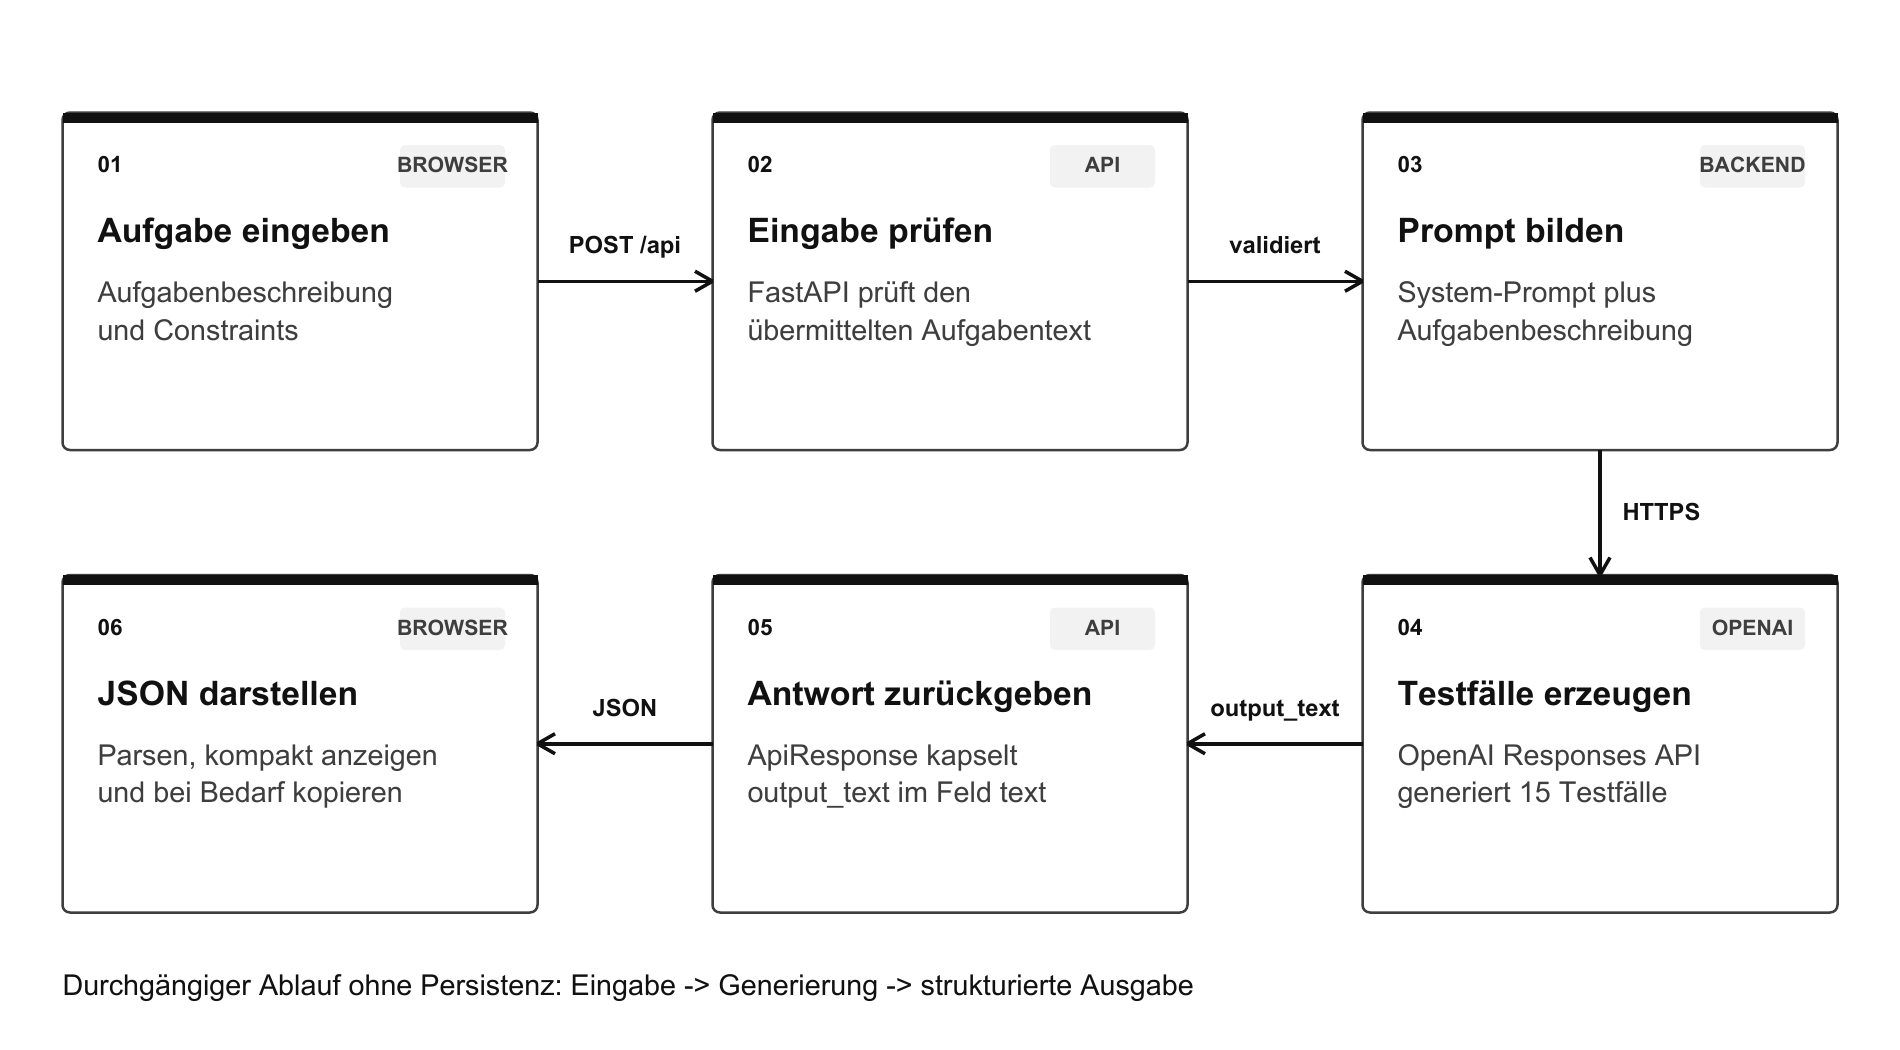
\includegraphics[width=0.8\textwidth]{assets/systemablauf.png}
    \caption{Systemablauf innerhalb der Webanwendung (Eigene Darstellung unter Verwendung von ChatGPT) \cite{openai_sol_2026}}
    \label{fig:systemablauf}
\end{figure}

Abbildung~\ref{fig:architektur} stellt wiederum den technischen Aufbau des Assistenzsystems dar. 

\begin{figure}[h]
    \centering
    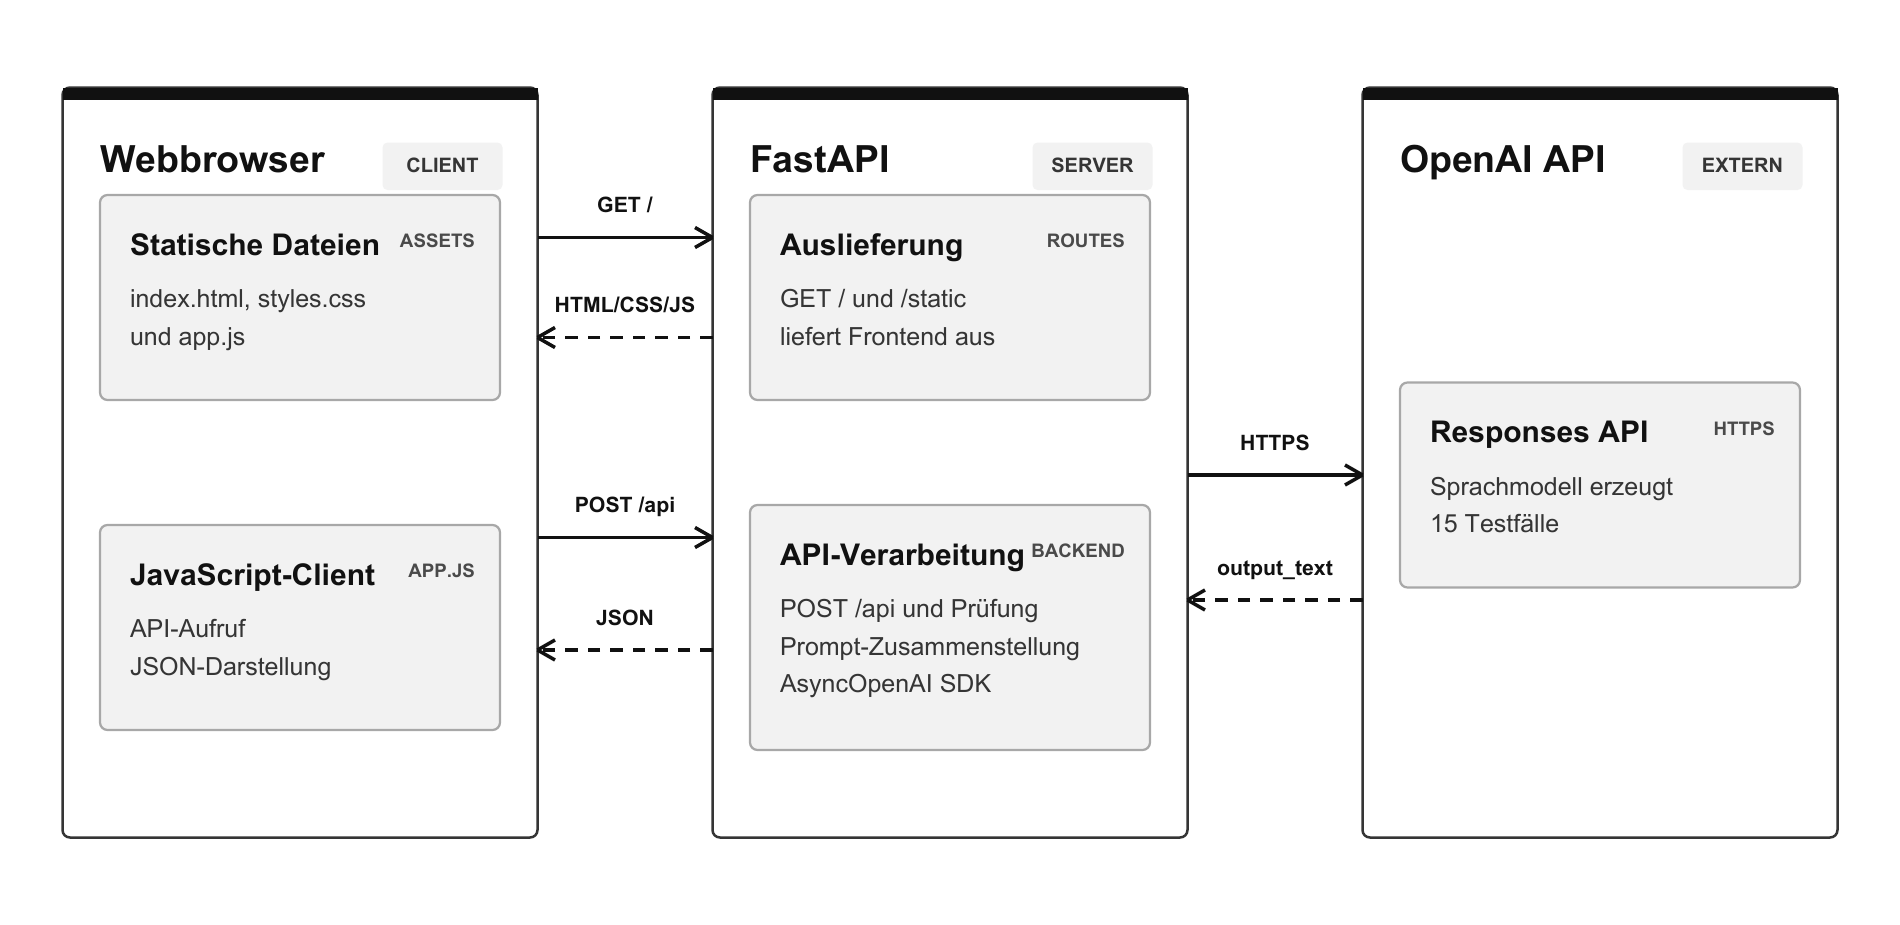
\includegraphics[width=0.8\textwidth]{assets/architektur.png}
    \caption{Architektur der Webanwendung (Eigene Darstellung unter Verwendung von ChatGPT) \cite{openai_sol_2026}}
    \label{fig:architektur}
\end{figure}

Die Anwendung besteht aus einem mit Python und dem Framework FastAPI \cite{fastapi_documentation}
realisierten Backend sowie einer mit \acs{HTML}, \acs{CSS} und JavaScript umgesetzten Benutzeroberfläche (Anhang~\ref{anhang:web-ui}). Beide Bestandteile werden gemeinsam innerhalb eines Serverprozesses 
betrieben. Über die Route \texttt{GET /} stellt das Backend die statischen Dateien der Benutzeroberfläche bereit und liefert sie an den Browser aus.
Die Benutzeroberfläche ermöglicht die Eingabe einer natürlichsprachlichen Programmieraufgabe und sendet diese anschließend über eine \acs{HTTP}-POST-Anfrage an 
den Endpunkt \texttt{POST /api}. Dort befindet sich die serverseitige Logik zur Verarbeitung der Anfrage und zur Generierung der Testfälle. Der Endpunkt übermittelt 
die aufbereitete Aufgabenbeschreibung an das verwendete Large Language Model und gibt dessen Antwort anschließend an die Benutzeroberfläche im Browser zurück, wo die 
generierten Testfälle dargestellt werden.

\subsection{Aufbau des System-Prompts}
Um dem \ac{LLM} mehr Kontext und klare Vorgaben zu geben, wird jeder Anfrage ein einheitlicher und vorab festgelegter System-Prompt beigefügt.
Dieser stellt eine wichtige Möglichkeit dar, das Verhalten des Modells und damit die Qualität der generierten Testfälle gezielt zu beeinflussen \cite{santana_software_2025}.
Die vom Nutzer eingegebene Aufgabenbeschreibung wird davon getrennt als Benutzernachricht
übermittelt. Diese Trennung verhindert, dass Instruktionen zur Rolle des \ac{LLM}s, zum
Ausgabeformat und zu den Qualitätsanforderungen bei jeder Anfrage erneut durch
die Benutzeroberfläche bereitgestellt werden müssen. Gleichzeitig sorgt sie
für ein einheitliches experimentelles Vorgehen, da alle Aufgaben unter
denselben Prompt-Bedingungen verarbeitet werden.

Der System-Prompt setzt sich konzeptionell aus fünf Bestandteilen zusammen:

\begin{enumerate}
    \item \textbf{Rollenbeschreibung:} Das Modell wird als Assistenzsystem zur
          Generierung von Black-Box-Testfällen aus natürlichsprachlichen
          Programmieraufgaben definiert. Dadurch wird die Aufgabe des Modells
          eingegrenzt und klar beschrieben.
    \item \textbf{Generierungsziel:} Für die übergebene Aufgabe sollen genau
          15 Testfälle einschließlich des jeweils erwarteten korrekten Outputs
          erzeugt werden.
    \item \textbf{Abdeckungsanforderung:} Das Modell wird angewiesen, typische
          Fehler und Randfälle zu berücksichtigen. Die Testfälle sollen so
          gewählt werden, dass fehlerhafte Implementierungen möglichst
          erkannt werden. Damit wird neben gewöhnlichen Eingaben explizit
          eine Edge-Case-Abdeckung gefordert.
    \item \textbf{Gültigkeitsbedingungen:} Alle in der Aufgabenbeschreibung
          genannten Eingabeeinschränkungen (Constraints) sind zwingend einzuhalten. Eingabewerte
          außerhalb der erlaubten Bereiche sollen ausgeschlossen werden. Wenn die Aufgabe 
          Beispieltestfälle enthält, dürfen diese nicht erneut verwendet werden.
          Diese Vorgaben sollen sowohl unzulässige Eingaben als auch
          eine künstliche Verbesserung der Abdeckung durch kopierte Beispiele
          vermeiden.
    \item \textbf{Ausgabevertrag:} Die Antwort des \ac{LLM}s soll ausschließlich aus einem
          gültigen \acs{JSON}-Objekt bestehen. Jeder einzelne Testfall enthält die für die
          jeweilige Funktionssignatur erforderlichen Eingabevariablen und das
          Feld \texttt{expected}, welches das vom Modell erwartete Ergebnis speichert.
\end{enumerate}

Der vollständige System-Prompt kann Anhang~\ref{anhang:system-prompt} entnommen werden.

Trotz der präzisen Vorgaben stellt der Prompt keine formale Garantie für ein 
gültiges Ausgabeformat, eingehaltene Constraints oder fachlich korrekte Sollwerte dar.
Wie im vorherigen Kapitel beschrieben, erzeugt ein \ac{LLM} seine Antwort auf Basis 
von Wahrscheinlichkeitsverteilungen und überführt die
beschriebenen Funktionalitäten nicht zwangsläufig in korrekte Ausgaben. 
Aus diesem Grund werden die generierten Testfälle in der anschließenden Evaluation zunächst mit einer
korrekten Referenzimplementierung validiert. Erst nach Ausschluss
unzulässiger Eingaben und fehlerhafter Sollwerte wird beurteilt, ob die
verbleibenden Testfälle bewusst fehlerhafte Implementierungen erkennen.

\newpage